\documentclass[tikz]{standalone}
%
%------------------------- formatting --------------------------%
% fonts
\usepackage{textcomp}
% set font shape helvetica
\usepackage[scaled=0.92]{helvet}
\renewcommand{\familydefault}{\sfdefault}
%
\usetikzlibrary{calc, arrows.meta}
\usepackage{ifthen}
%
\newcommand{\PicLab}{}
%
\newlength{\PSep}
\newlength{\YOffSet}
\newlength{\tmp}
\newlength{\tmpp}
\newlength{\PicWidth}
%
\begin{document}
	%	
	\setlength{\PSep}{0.3ex}
	\setlength{\PicWidth}{4cm}
	%	
	\normalsize % font size
	%
	\begin{tikzpicture}[Label/.style={font=\bfseries, inner sep=0ex, xshift=1ex, anchor=west}]
		%
		% =================================================
		% Myc
		\path (0,0) node[inner sep=0ex] (Myc) {
\includegraphics[width=\PicWidth]{Cropped/Myc.jpg}};
		% frame
		\draw (Myc.north west) rectangle (Myc.south east);
		% label
		\draw (Myc.east) node[Label] (MycLabel) {$\alpha$-Myc};
		% %---------------------------- grid -----------------------------%
		% \renewcommand{\PicLab}{Myc}
		% % x
		% \foreach \x in {0,10,...,100}{
		% 	\draw[red, opacity=0.5] ($(\PicLab.north west)!\x/100!(\PicLab.north east)$) node[anchor=south,font={\tiny}] {\x} -- ($(\PicLab.south west)!\x/100!(\PicLab.south east)$);
		% }
		% \foreach \x in {5,15,...,95}{
		% 	\draw[red, opacity=0.25] ($(\PicLab.north west)!\x/100!(\PicLab.north east)$) -- ($(\PicLab.south west)!\x/100!(\PicLab.south east)$);
		% }
		% % y
		% \foreach \y in {0,10,...,100}{
		% 	\draw[red, opacity=0.5] ($(\PicLab.north west)!\y/100!(\PicLab.south west)$) node[anchor=east,font={\tiny}] {\y} -- ($(\PicLab.north east)!\y/100!(\PicLab.south east)$);
		% }
		% \foreach \y in {5,15,...,95}{
		% 	\draw[red, opacity=0.25] ($(\PicLab.north west)!\y/100!(\PicLab.south west)$) -- ($(\PicLab.north east)!\y/100!(\PicLab.south east)$);
		% }
		%--------------------------- labels ----------------------------%
		\begin{scope}[every node/.style={inner sep=0.5ex}]
			% 
			% genotype
			\pgfmathsetmacro{\Start}{0.15}
			\pgfmathsetmacro{\Sep}{0.18}
			\path (Myc.north east) node[anchor=south west] (L) {\strut};
			\foreach[count=\i from 1] \x in {\textit{fun30$\Delta$}, \textit{FUN30-9MYC}, 1:100, 1:10, undil.}{
				\pgfmathsetmacro{\y}{\Start+(\i-1)*\Sep}
				% alternating offset
				\pgfmathtruncatemacro{\rest}{mod(\i,2)}
				\ifthenelse{\rest = 0}{\setlength{\YOffSet}{0ex}}{\setlength{\YOffSet}{0ex}}
				\path ($(Myc.north west)!\y!(Myc.north east)$) coordinate (x);
				\path ($(x|-L.south)+(0,\YOffSet)$) node[anchor=south west, rotate=45] (L\i) {\x};
			}
			% top label
			\setlength{\tmp}{0ex}
			\setlength{\tmpp}{-0.25ex}
			\draw ($(L3.north east)+(-\tmp,\tmpp)$) coordinate (x) -- ($(x-|L5.east)+(\tmp,0)$) node[midway, anchor=south west, rotate=45] {\textit{pTDH3-FUN30-9MYC}};
			%
			% kDa
			\draw ($(Myc.north west)!0.17!(Myc.south west)-(1\PSep,0)$) -- ++(-2ex, 0ex) node[anchor=east] {250 kDa};
			\draw ($(Myc.north west)!0.64!(Myc.south west)-(1\PSep,0)$) -- ++(-2ex, 0ex) node[anchor=east] {150 kDa};
		\end{scope}
		%
		% =================================================
		% Myc long
		\path (Myc.south) ++(0,-0.5ex) node[inner sep=0ex, anchor=north] (Myc) {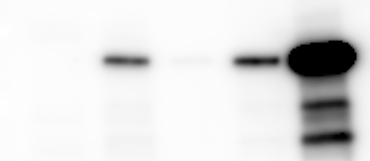
\includegraphics[width=\PicWidth]{Cropped/Myc_long.jpg}};
		% frame
		\draw (Myc.north west) rectangle (Myc.south east);
		% label
		\draw (Myc.east) node[Label, align=left] (MycLabel) {$\alpha$-Myc\\\normalfont(long exp.)};
		% %---------------------------- grid -----------------------------%
		% \renewcommand{\PicLab}{Myc}
		% % x
		% \foreach \x in {0,10,...,100}{
		% 	\draw[red, opacity=0.5] ($(\PicLab.north west)!\x/100!(\PicLab.north east)$) node[anchor=south,font={\tiny}] {\x} -- ($(\PicLab.south west)!\x/100!(\PicLab.south east)$);
		% }
		% \foreach \x in {5,15,...,95}{
		% 	\draw[red, opacity=0.25] ($(\PicLab.north west)!\x/100!(\PicLab.north east)$) -- ($(\PicLab.south west)!\x/100!(\PicLab.south east)$);
		% }
		% % y
		% \foreach \y in {0,10,...,100}{
		% 	\draw[red, opacity=0.5] ($(\PicLab.north west)!\y/100!(\PicLab.south west)$) node[anchor=east,font={\tiny}] {\y} -- ($(\PicLab.north east)!\y/100!(\PicLab.south east)$);
		% }
		% \foreach \y in {5,15,...,95}{
		% 	\draw[red, opacity=0.25] ($(\PicLab.north west)!\y/100!(\PicLab.south west)$) -- ($(\PicLab.north east)!\y/100!(\PicLab.south east)$);
		% }
		%--------------------------- labels ----------------------------%
		\begin{scope}[every node/.style={inner sep=0.5ex}]
			% kDa
			\draw ($(Myc.north west)!0.17!(Myc.south west)-(1\PSep,0)$) -- ++(-2ex, 0ex) node[anchor=east] {250 kDa};
			\draw ($(Myc.north west)!0.64!(Myc.south west)-(1\PSep,0)$) -- ++(-2ex, 0ex) node[anchor=east] {150 kDa};
		\end{scope}
		%
		% =================================================
		% Pgk1
		\path (Myc.south) ++(0,-1.5ex) node[inner sep=0ex, anchor=north] (Pgk1) {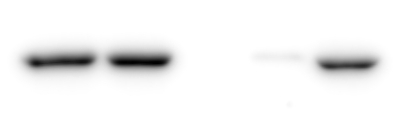
\includegraphics[width=\PicWidth]{Cropped/Pgk1.jpg}};
		% frame
		\draw (Pgk1.north west) rectangle (Pgk1.south east);
		% label
		\draw (Pgk1.east) node[Label] {$\alpha$-Pgk1};
		% %---------------------------- grid -----------------------------%
		% \renewcommand{\PicLab}{Pgk1}
		% % x
		% \foreach \x in {0,10,...,100}{
		% 	\draw[red, opacity=0.5] ($(\PicLab.north west)!\x/100!(\PicLab.north east)$) node[anchor=south,font={\tiny}] {\x} -- ($(\PicLab.south west)!\x/100!(\PicLab.south east)$);
		% }
		% \foreach \x in {5,15,...,95}{
		% 	\draw[red, opacity=0.25] ($(\PicLab.north west)!\x/100!(\PicLab.north east)$) -- ($(\PicLab.south west)!\x/100!(\PicLab.south east)$);
		% }
		% % y
		% \foreach \y in {0,10,...,100}{
		% 	\draw[red, opacity=0.5] ($(\PicLab.north west)!\y/100!(\PicLab.south west)$) node[anchor=east,font={\tiny}] {\y} -- ($(\PicLab.north east)!\y/100!(\PicLab.south east)$);
		% }
		% \foreach \y in {5,15,...,95}{
		% 	\draw[red, opacity=0.25] ($(\PicLab.north west)!\y/100!(\PicLab.south west)$) -- ($(\PicLab.north east)!\y/100!(\PicLab.south east)$);
		% }
		%--------------------------- labels ----------------------------%
		\begin{scope}[every node/.style={inner sep=0.5ex}]
			% 
			% kDa
			\draw ($(Pgk1.north west)!0.23!(Pgk1.south west)-(1\PSep,0)$) -- ++(-2ex, 0ex) node[anchor=east] {50 kDa};
			\draw ($(Pgk1.north west)!0.89!(Pgk1.south west)-(1\PSep,0)$) -- ++(-2ex, 0ex) node[anchor=east] {37 kDa};
			%
		\end{scope}
		%
	\end{tikzpicture}
	%
\end{document}